\documentclass[xcolor=x11names,compress,mathserif]{beamer}

\newcommand{\hackspace}{\hspace{4.2mm}}
\newcommand{\showstudent}[1]{}
\newcommand\hmmax{0}
\newcommand\bmmax{0}


\usepackage{../includes/MarkMathCmds}





% talk/author information
\newcommand{\authorname}{Mark van der Wilk}
\newcommand{\authoremail}{m.vdwilk@imperial.ac.uk}
\newcommand{\authoraffiliation}{
  Department of Computing\\Imperial
  College London}
\newcommand{\authortwitter}{markvanderwilk}
\newcommand{\slidesettitle}{\imperialBlue{Bayesian Linear Regression}}
\newcommand{\footertitle}{Measuring Generalisation}
\newcommand{\location}{Imperial College London}
\newcommand{\talkDate}{November 16, 2021}



\date{\imperialGray{\talkDate}}

% load defaults
\input{../includes/header.tex}


\input{../includes/titlepage.tex}
\linespread{1.2} 



\begin{frame}{Last time}
\begin{itemize}
\item Discussed the principle of Bayesian inference
\item Skill: Compute posteriors
\begin{itemize}
\item Example: Coin flipping (continuous latent, discrete obs)
\item Example: Noisy communication (discrete latent, continuous obs)
\end{itemize}
\item Introduced: Noisy communication with Gaussian prior on signal.
\item Skill: Gaussian conditioning.
\end{itemize}

\pause

\vspace{0.5cm}
To help with clarity, I made a notebook of figures to clarify last Friday's lecture (\texttt{l10-bayes-voltage.ipynb}). Do carefully look at it.
\end{frame}

\begin{frame}{Gaussian Conditioning}
Many important models are \emph{Linear Gaussian Models}.
\begin{itemize}
\item Bayesian Linear Regression
\item Factor Analysis / PCA / Linear Autoencoders
\item Kalman filters (time series)
\end{itemize} \pause

\vspace{0.3cm}
Special because:
\begin{itemize}
\item You can compute posteriors in closed form \\ {\tiny(\emph{closed form} means that you can express some solution in terms of typical functions $\log$, $\sin$, etc...)}
\item This is rare in Bayesian inference!
\end{itemize} \pause

\begin{center}
Key skill: Conditioning in Gaussian distributions.
\end{center}
\end{frame}


\begin{frame}{Example: Noisy analogue communication}
Similar set-up to before.
\begin{align}
p(s) &= \NormDist{s; 0, 1} && \text{Assume a prior on source voltage.} \\
p(v|s) &= \NormDist{v; s, \sigma^2} && \text{Assumptions about the channel.}
\end{align}

\vspace{0.5cm} \pause

We are interested in our posterior belief on $S$:
\begin{align}
p(s|v) &= \frac{p(v|s)p(v)}{p(v)} \\
&= \frac{p(v,s)}{\int p(v,s) \mathrm ds} && \text{Alternative formulation (sum/prod rules)}
\end{align}
\end{frame}

\begin{frame}{Two formulations, two methods of solving}
Both share the same goal:
\begin{enumerate}
\item Find an expression of the posterior density that you can directly implement (closed-form)
\item Express posterior as a known standard type of distribution
\end{enumerate}
\end{frame}


\begin{frame}[t]{Method 1: Crunching through densities}
One method always works: Crunching through the densities.

{\tiny We only care about terms that depend on $s$, since we know that a distribution has to normalise to 1!}
\begin{align}
p(s|v) &\,\propto\, p(v|s)p(s) \\
&= \NormDist{v; s, \sigma^2}\NormDist{s; 0, 1} \\
&\propto\, \exp\left(-\frac{(v-s)^2}{2\sigma^2}\right)\exp\left(-\frac{s^2}{2}\right) \\
&= \exp\left(-\frac{v^2}{2\sigma^2} + \frac{sv}{\sigma^2} - \frac{s^2}{2\sigma^2} - \frac{s^2}{2}\right) \\
&\propto\, \exp\left(-\frac{1 + \sigma^2}{2\sigma^2}s^2 + \frac{v}{\sigma^2}s \right)
\end{align}
\end{frame}


\begin{frame}[t]{Method 1: Equating coefficients}
\begin{gather}
\NormDist{s; a, b} = c\cdot\exp\left(-\frac{1}{2b}x^2 + \frac{a}{b}x\right) \\
\implies b = \frac{\sigma^2}{1+\sigma^2} \\
\implies a = \frac{1}{1+\sigma^2}v \\
\implies p(s|v) = \NormDist{s; \frac{1}{1+\sigma^2}v, \frac{\sigma^2}{1+\sigma^2}}
\end{gather} \pause
\begin{itemize}
\item Best guess (mode/mean) is more conservative than MaxLik (biased towards the mean of the prior)
\item Variance tends to zero as $\sigma^2 \to 0$
\end{itemize}
\end{frame}


\begin{frame}[t]{Method 2: Joint and Conditioning Formula}
Alter: we could find the joint first, and then evaluate along a line
\begin{figure}
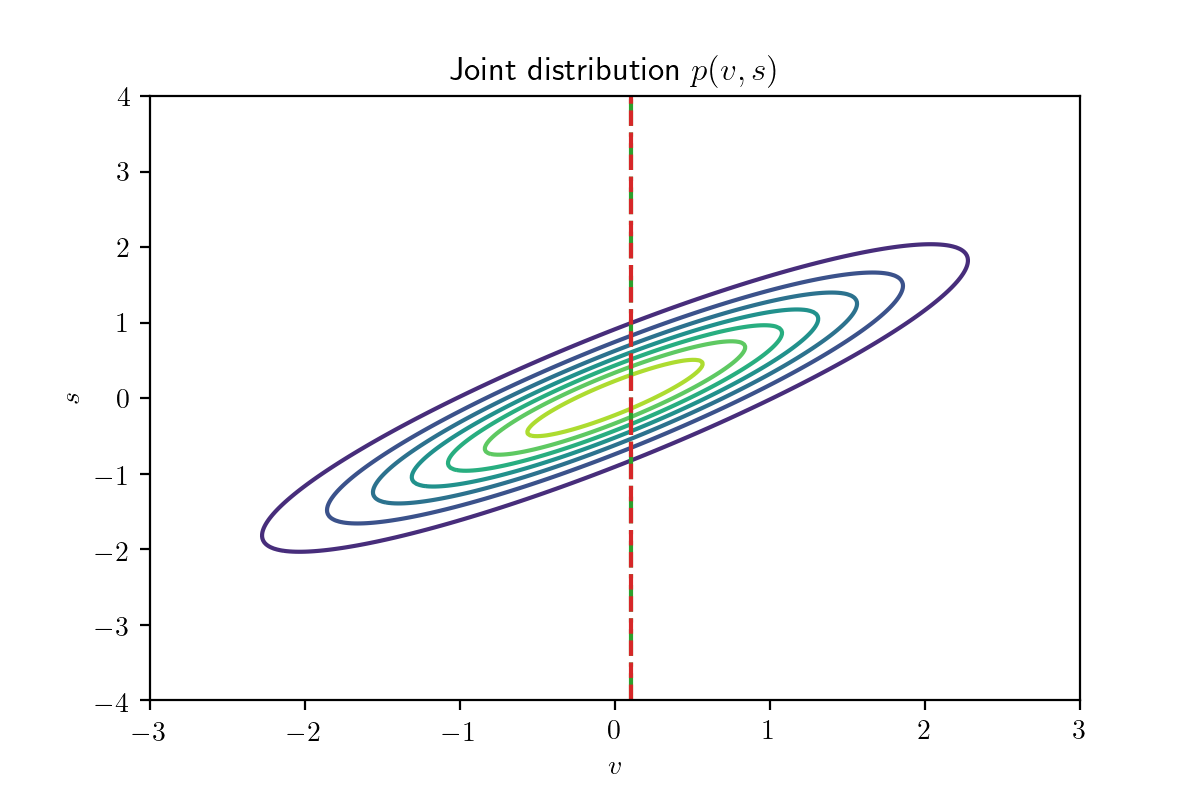
\includegraphics[width = 0.7\hsize]{./figures-bayesgauss/joint-gauss.png}
\end{figure}
\end{frame}

\begin{frame}{Method 2: Gaussian Conditioning Formula}
For a joint Gaussian density
\begin{align}
p(x, y) = \NormDist{\begin{bmatrix}x \\ y\end{bmatrix}; \begin{bmatrix}a \\ b \end{bmatrix}, \begin{bmatrix}A & B \\ B & C\end{bmatrix}}
\end{align}
we have the conditional
\begin{align}
p(y|x) = \NormDist{y; \frac{B}{A}(x-a) + b, C - \frac{B^2}{A}}
\end{align}
\end{frame}


\begin{frame}{Linear Gaussian Model}
Linear-Gaussian model: \pause
\begin{itemize}
\item All RVs are conditionally Gaussian. \pause
\item Conditional means can depend \emph{linearly} on other RVs. \pause
\item Can always rewrite as linear combination of independent Gaussian RVs. \pause
\item Linear transformations of Gaussians are still Gaussian (earlier lectures / exercise) \pause
\item This gives an easy way of finding the joint.
\end{itemize}

\end{frame}


\begin{frame}{Method 2: Example}
Set-up:
\begin{align}
p(s) &= \NormDist{s; 0, 1} && \text{Assume a prior on source voltage.} \\
p(v|s) &= \NormDist{v; s, \sigma^2} && \text{Assumptions about the channel.}
\end{align}

\pause

Write as linear transform, use expectation identities to find means and covariances:
\begin{align}
\onslide<2->{\begin{bmatrix}s \\ v\end{bmatrix} = \begin{bmatrix}\mathrm 1 & 0 \\ 1 & 1\end{bmatrix}\begin{bmatrix}s \\ \epsilon\end{bmatrix}} \\
\onslide<3->{\Exp{s,\epsilon}{v} = \Exp{s,\epsilon}{s + \epsilon} = \Exp{s}{s} + \Exp{\epsilon}{\epsilon} = 0} \\
\onslide<4->{\Var{s,\epsilon}{v} = \Var{s,\epsilon}{s + \epsilon} = \Var{s}{s} + \Exp{\epsilon}{\epsilon} = 1 + \sigma^2 && \text{Indep.}} \\
\onslide<5->{\Cov{s,\epsilon}{s,v} = \Exp{s,\epsilon}{(s+\epsilon)s} = \Exp{s}{s}\Exp{\epsilon}{\epsilon} + \Exp{\epsilon}{s^2} && \text{Indep.}} \\
\onslide<6->{  = 0 + \Var{s}{s} = 1 && \Exp{\epsilon}{\epsilon} = 0}
\end{align}
\end{frame}

\begin{frame}[t]{Method 2: Example continued}
Given the means, variances and covariances we have computed, we can fill in the full joint:
\begin{align}
p(s, v) = \NormDist{\begin{bmatrix}v \\ s\end{bmatrix}; \begin{bmatrix}0 \\ 0 \end{bmatrix}, \begin{bmatrix}1 + \sigma^2 & 1 \\ 1 & 1\end{bmatrix}}
\end{align} \pause

We can now apply the Gaussian conditioning formula (make sure $s,v$ are the right way round):
\begin{align}
p(s|v) &= \NormDist{s; \frac{\sigma^2}{1+\sigma^2}v, 1 - \frac{1}{1+\sigma^2}} \\
&= \NormDist{s; \frac{\sigma^2}{1+\sigma^2}v, \frac{\sigma^2}{1+\sigma^2}}
\end{align}
\end{frame}

\begin{frame}{Conclusion}
Gaussian conditioning:
\begin{itemize}
\item Method 1: Equating coefficients
\item Method 2: Finding joint, using conditioning formula
\end{itemize}
\end{frame}




\end{document}
%%% Local Variables: 
%%% mode: latex
%%% TeX-master: t
%%% End: 
